% Created 2023-08-25 vie 22:20
% Intended LaTeX compiler: pdflatex
\documentclass[11pt]{article}
\usepackage[utf8]{inputenc}
\usepackage[T1]{fontenc}
\usepackage{graphicx}
\usepackage{grffile}
\usepackage{longtable}
\usepackage{wrapfig}
\usepackage{rotating}
\usepackage[normalem]{ulem}
\usepackage{amsmath}
\usepackage{textcomp}
\usepackage{amssymb}
\usepackage{capt-of}
\usepackage{hyperref}
\usepackage{../modern}
\bibliography{fuentes.bib}
\raggedbottom
\setcounter{secnumdepth}{3}
\author{Luis Eduardo Galindo Amaya (1274895)}
\date{16 de Agosto 2023}
\title{Práctica 1: Principios de Diseño de Tecnologías Emergentes}
\hypersetup{
 pdfauthor={Luis Eduardo Galindo Amaya (1274895)},
 pdftitle={Práctica 1: Principios de Diseño de Tecnologías Emergentes},
 pdfkeywords={},
 pdfsubject={},
 pdfcreator={Emacs 27.1 (Org mode 9.3)}, 
 pdflang={Spanish}}
\begin{document}

\modentitlepage{../images/escudo-uabc-2022-1-tinta-pos.png}

\tableofcontents
\pagebreak

\datasection{Individual}

\section{Introducción}
\label{sec:org4ea7af9}
Una parte clave del diseño de aplicaciones modernas es la interfaz gráfica. 
Esta interfaz hace que sea más fácil para los usuarios utilizar la aplicación, 
lo que resulta en una mayor aceptación y un tiempo de aprendizaje más corto para
usar el software de manera efectiva. En esta práctica, exploraremos algunos
conceptos de diseño de interfaces a nivel de diseño y de experiencia de usuario.

\section{Investigación de usuarios}
\label{sec:org9c645bd}
\autocite{drachen2018games} La investigación de usuarios para videojuegos 
es un campo interdisciplinario de investigación que se enfoca en garantizar la 
óptima estabilidad y experiencia (UX) en los videojuegos\footnote{No lo pude encontrar enfocado a UI.}.

\begin{figure}[htbp]
\centering

\includegraphics[width=5cm]{images/iusuario.png}
\caption{Proceso de investigación de usuario.}
\end{figure}

\subsection{Objetivos del estudio de usuarios}
\label{sec:orge2ee2e6}
\autocite{Yépez_2021} Conocer los hábitos, actitudes, opiniones, deseos, 
necesidades, demandas y grado de satisfacción de los individuos en relación 
tanto de la información como con los servicios de los centros que se la 
proporcionan.

\section{Arquitectura de la información}
\label{sec:org81220c4}
\autocite{Rosenfeld_Morville_2002} La arquitectura de la información ayuda 
a nuestros usuarios a entender dónde están, qué han encontrado, qué pueden 
esperar y qué hay alrededor. Ayudamos a nuestros clientes a entender qué es 
posible.

\begin{figure}[htbp]
\centering

\includegraphics[width=5cm]{images/ai.png}
\caption{Enfoque de la Arquitectura de la información.}
\end{figure}

\subsection{Origen de la Arquitectura de la información}
\label{sec:org3589a1b}
\autocite{gonzales_2003} El término Arquitectura de la Información es un 
concepto utilizado en su forma más amplia para expresar el diseño, organización 
y distribución de los sistemas informáticos. Richard Saul Wurman acuñó el término
en 1976, y trabajó seriamente en la estructura de la información dentro de sus
publicaciones, como Information  Anxiety, Information Architects, y Information 
Design. A partir de esta fecha se ha ido extendiendo su uso dentro de las
publicaciones técnicas y de referencia, y hasta se ha creado un perfil 
laboral que comparte muchas habilidades de varias disciplinas.

\section{Diseño de Interfaz de Usuario (UI)}
\label{sec:org91bcf81}
\autocite{ovacen_2022} Una interfaz de usuario es la presentación visual de
la interacción entre un dispositivo con software, producto o servicio, y un
usuario. También llamado UI (User Interface) transforma ciertas señales, 
imágenes, símbolos o acciones de un sistema para hacerlas comprensibles al ser
humano. Una simplificación del concepto.

\begin{itemize}
\item La interfaz debe diseñarse con el objetivo de disminuir las necesidades del usuario para recordar acciones, resultados y elementos del pasado.
\item La visual preestablecida debe de ser coherente con el usuario común ¡reconocible! Además, debe de aparecer un elemento para «reiniciar» (restablecer valores originales).
\item Crear atajos que sean intuitivos y de fácil acceso.
\item Crear una interfaz visual donde los elementos más importantes se parezcan al mundo real.
\item La información debe ser revelada de manera progresiva.
\end{itemize}

\subsection{Fases del diseño de UI}
\label{sec:org170e85c}
\autocite{Alli_2022} Hablando en términos generales, diseñar interfaces de 
usuario es un proceso de descubrir cómo representar visualmente los 
componentes, cambios de estado e interacciones que un usuario enfrentará cuando 
interactúe con tus diseños en pantalla.

\subsubsection{1. Sketches}
\label{sec:org45c8a23}
Esta es la forma más rápida, económica y de menor compromiso para iniciar tus 
diseños. Permite plasmar las ideas de alto nivel y prioritarias que tienes en 
mente en el papel o la pantalla. Por lo general, estas son ideas capturadas de 
manera aproximada y si lucen bastante mal, entonces probablemente vas por el 
camino correcto.

\begin{figure}[htbp]
\centering
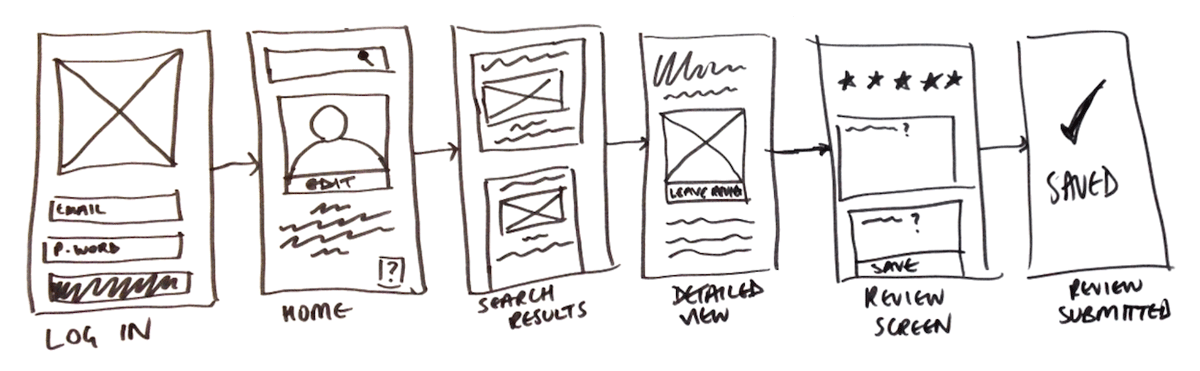
\includegraphics[width=9cm]{images/sketch.png}
\caption{Sketeches o 'low fidelity wireframe'}
\end{figure}

\subsubsection{2. Wireframes o Gray boxing}
\label{sec:orge4e02b2}
los wireframes de fidelidad media presentan representaciones más precisas de la 
disposición. Aunque aún evitan distracciones como imágenes o tipografía, se 
asigna más detalle a componentes específicos y las características se 
diferencian claramente entre sí.

\begin{figure}[htbp]
\centering
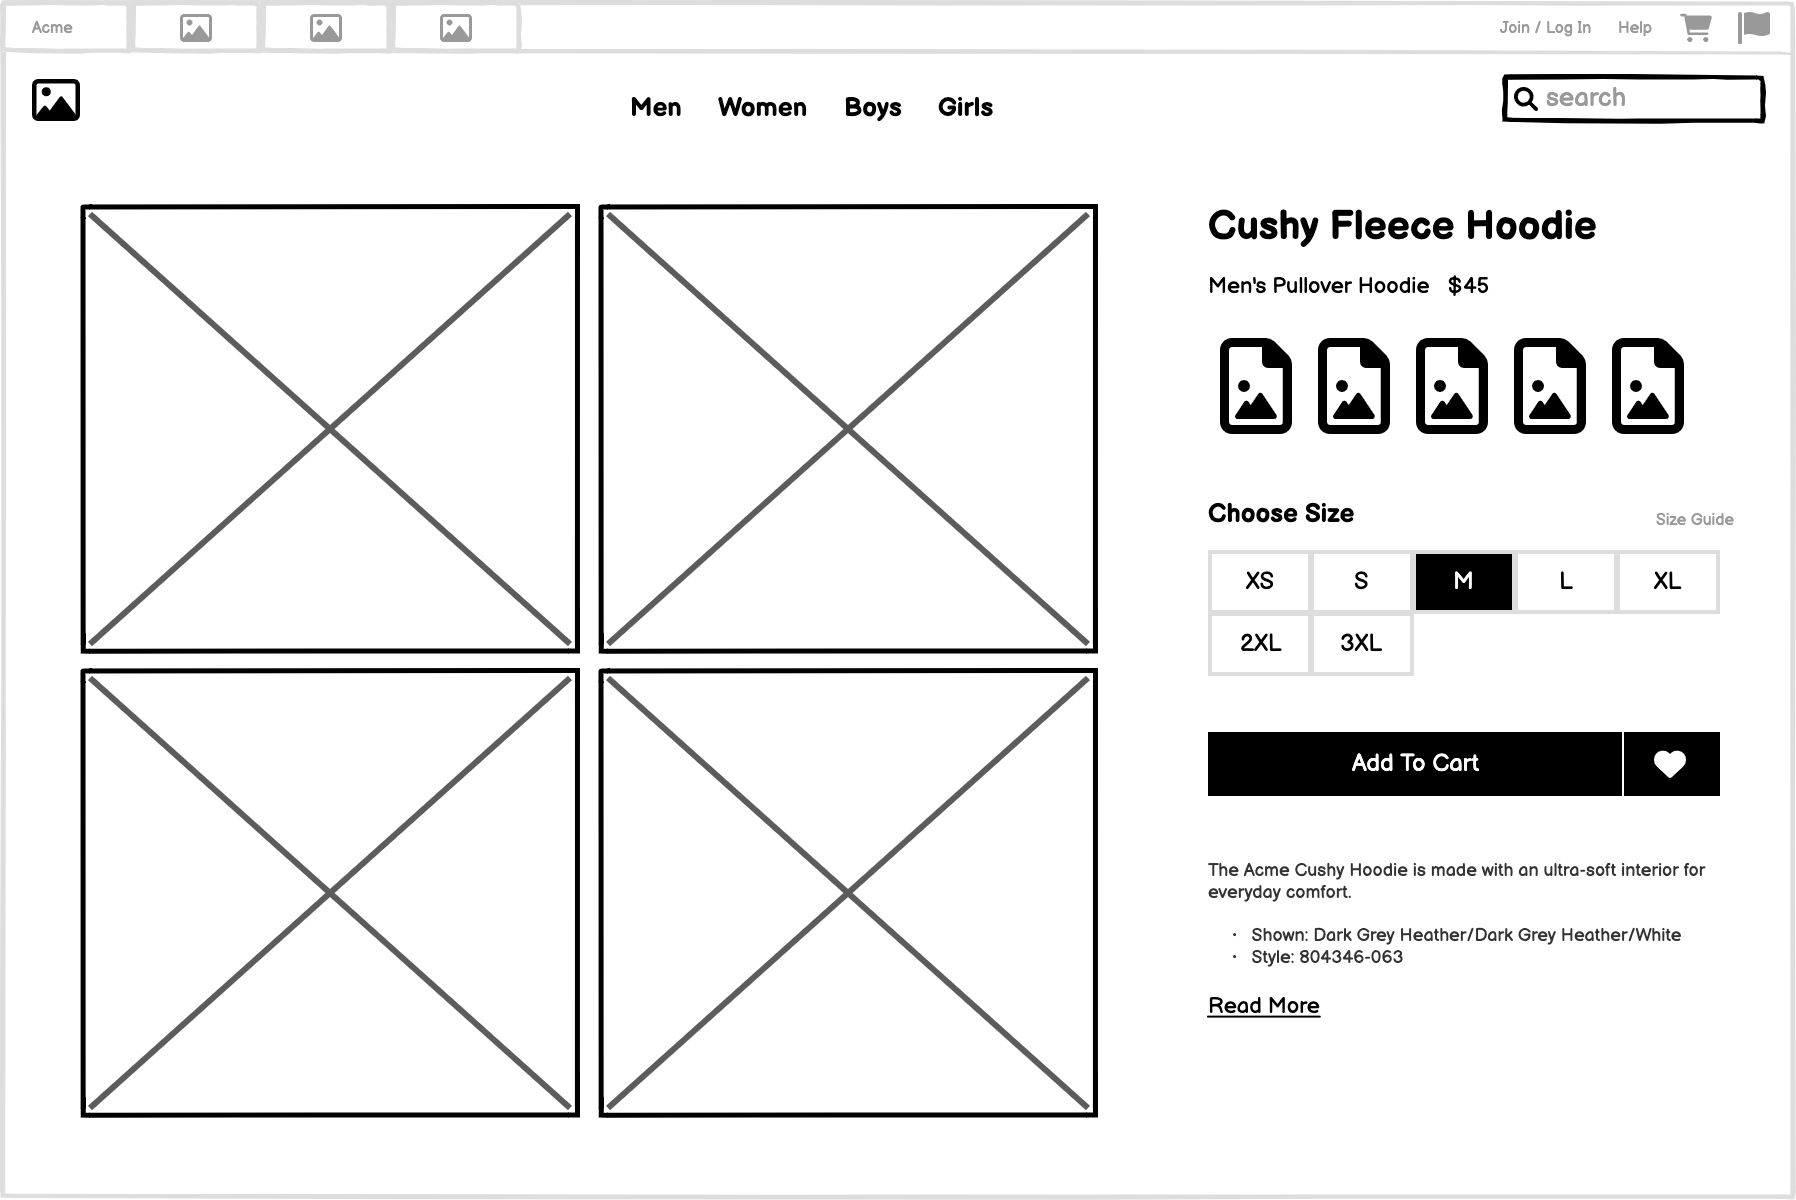
\includegraphics[width=7cm]{images/wireframe.png}
\caption{Ejemplo de un wireframe}
\end{figure}

\subsubsection{3. User Flows y Task flows}
\label{sec:orgf8dcda0}
¿Qué sucede cuando hacen clic en esto o si olvidan agregar cierta información
aquí? Se trata de comprender los modelos mentales del usuario y el modelo de tu
sistema, así como la coordinación de las vías y respuestas que proporcionará tu 
interfaz.

\begin{figure}[htbp]
\centering
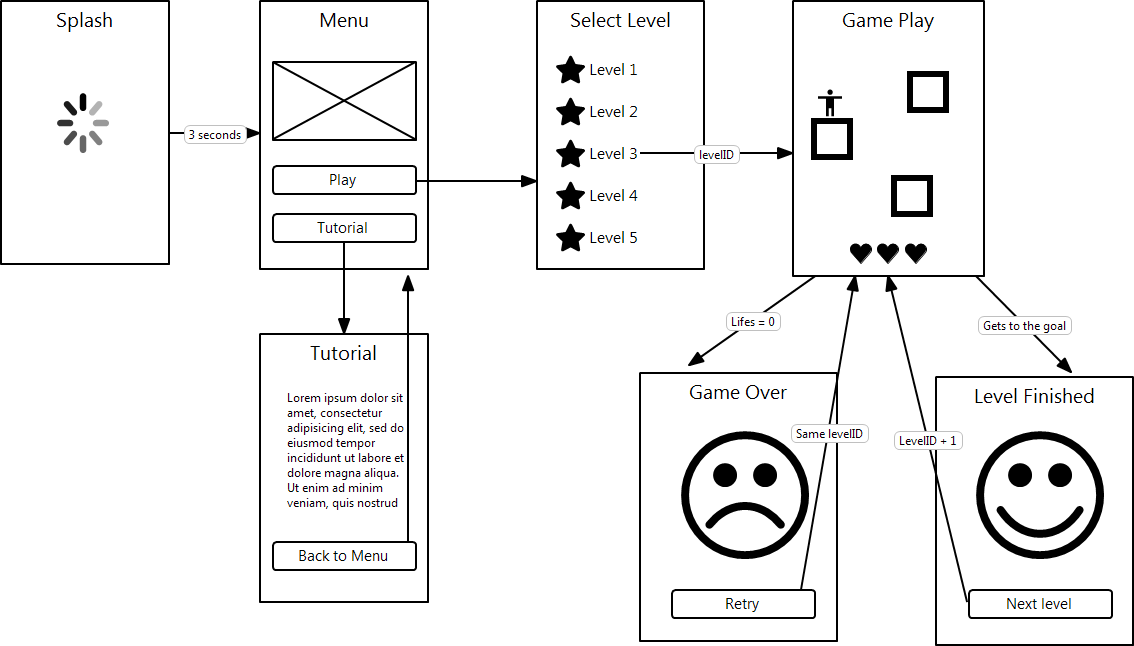
\includegraphics[width=9cm]{images/userflow.png}
\caption{Diagrama de flujo para la aplicación}
\end{figure}

\subsubsection{4. Diseños de alta fidelidad}
\label{sec:orgf012bbf}
Aquí es donde haces cada píxel tan perfecto y medido como puedas, y donde 
puedes añadir tu estética de marca única y elementos temáticos.

\begin{figure}[htbp]
\centering
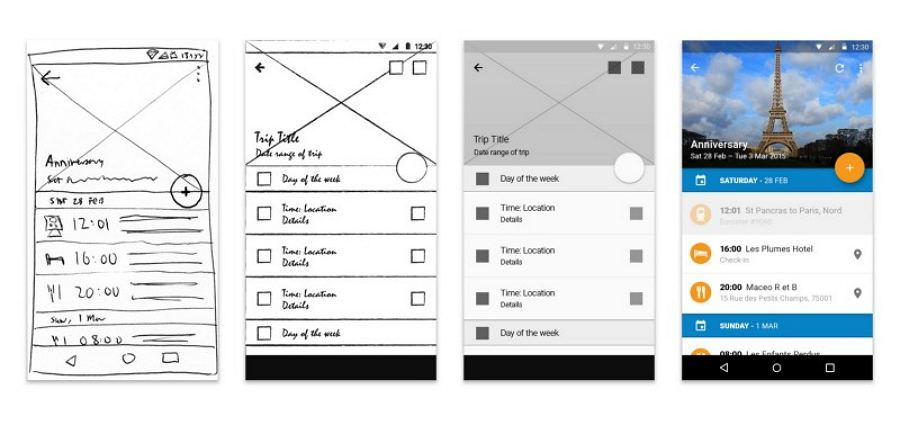
\includegraphics[width=13cm]{images/hightfidelity.jpg}
\caption{Desarrollo de la interfaz}
\end{figure}

\subsubsection{5. Prototipo}
\label{sec:orgcea648b}
Esto une todo y muestra cómo se espera que se vea y comporte la aplicación.


\subsection{Herramientas para diseño de UI}
\label{sec:org2cf6128}
\subsubsection{Whimsical.com}
\label{sec:org05b275c}
Whimsical es una herramienta para diseñar wireframes que permite a cualquier persona 
participar en el diseño de experiencia de usuario y crear esquemas, puede integrarse
con otros archivos como diagramas de flujo y mapas conceptuales además de funciones
simples para diseñar el flujo de la aplicación.

\begin{figure}[htbp]
\centering
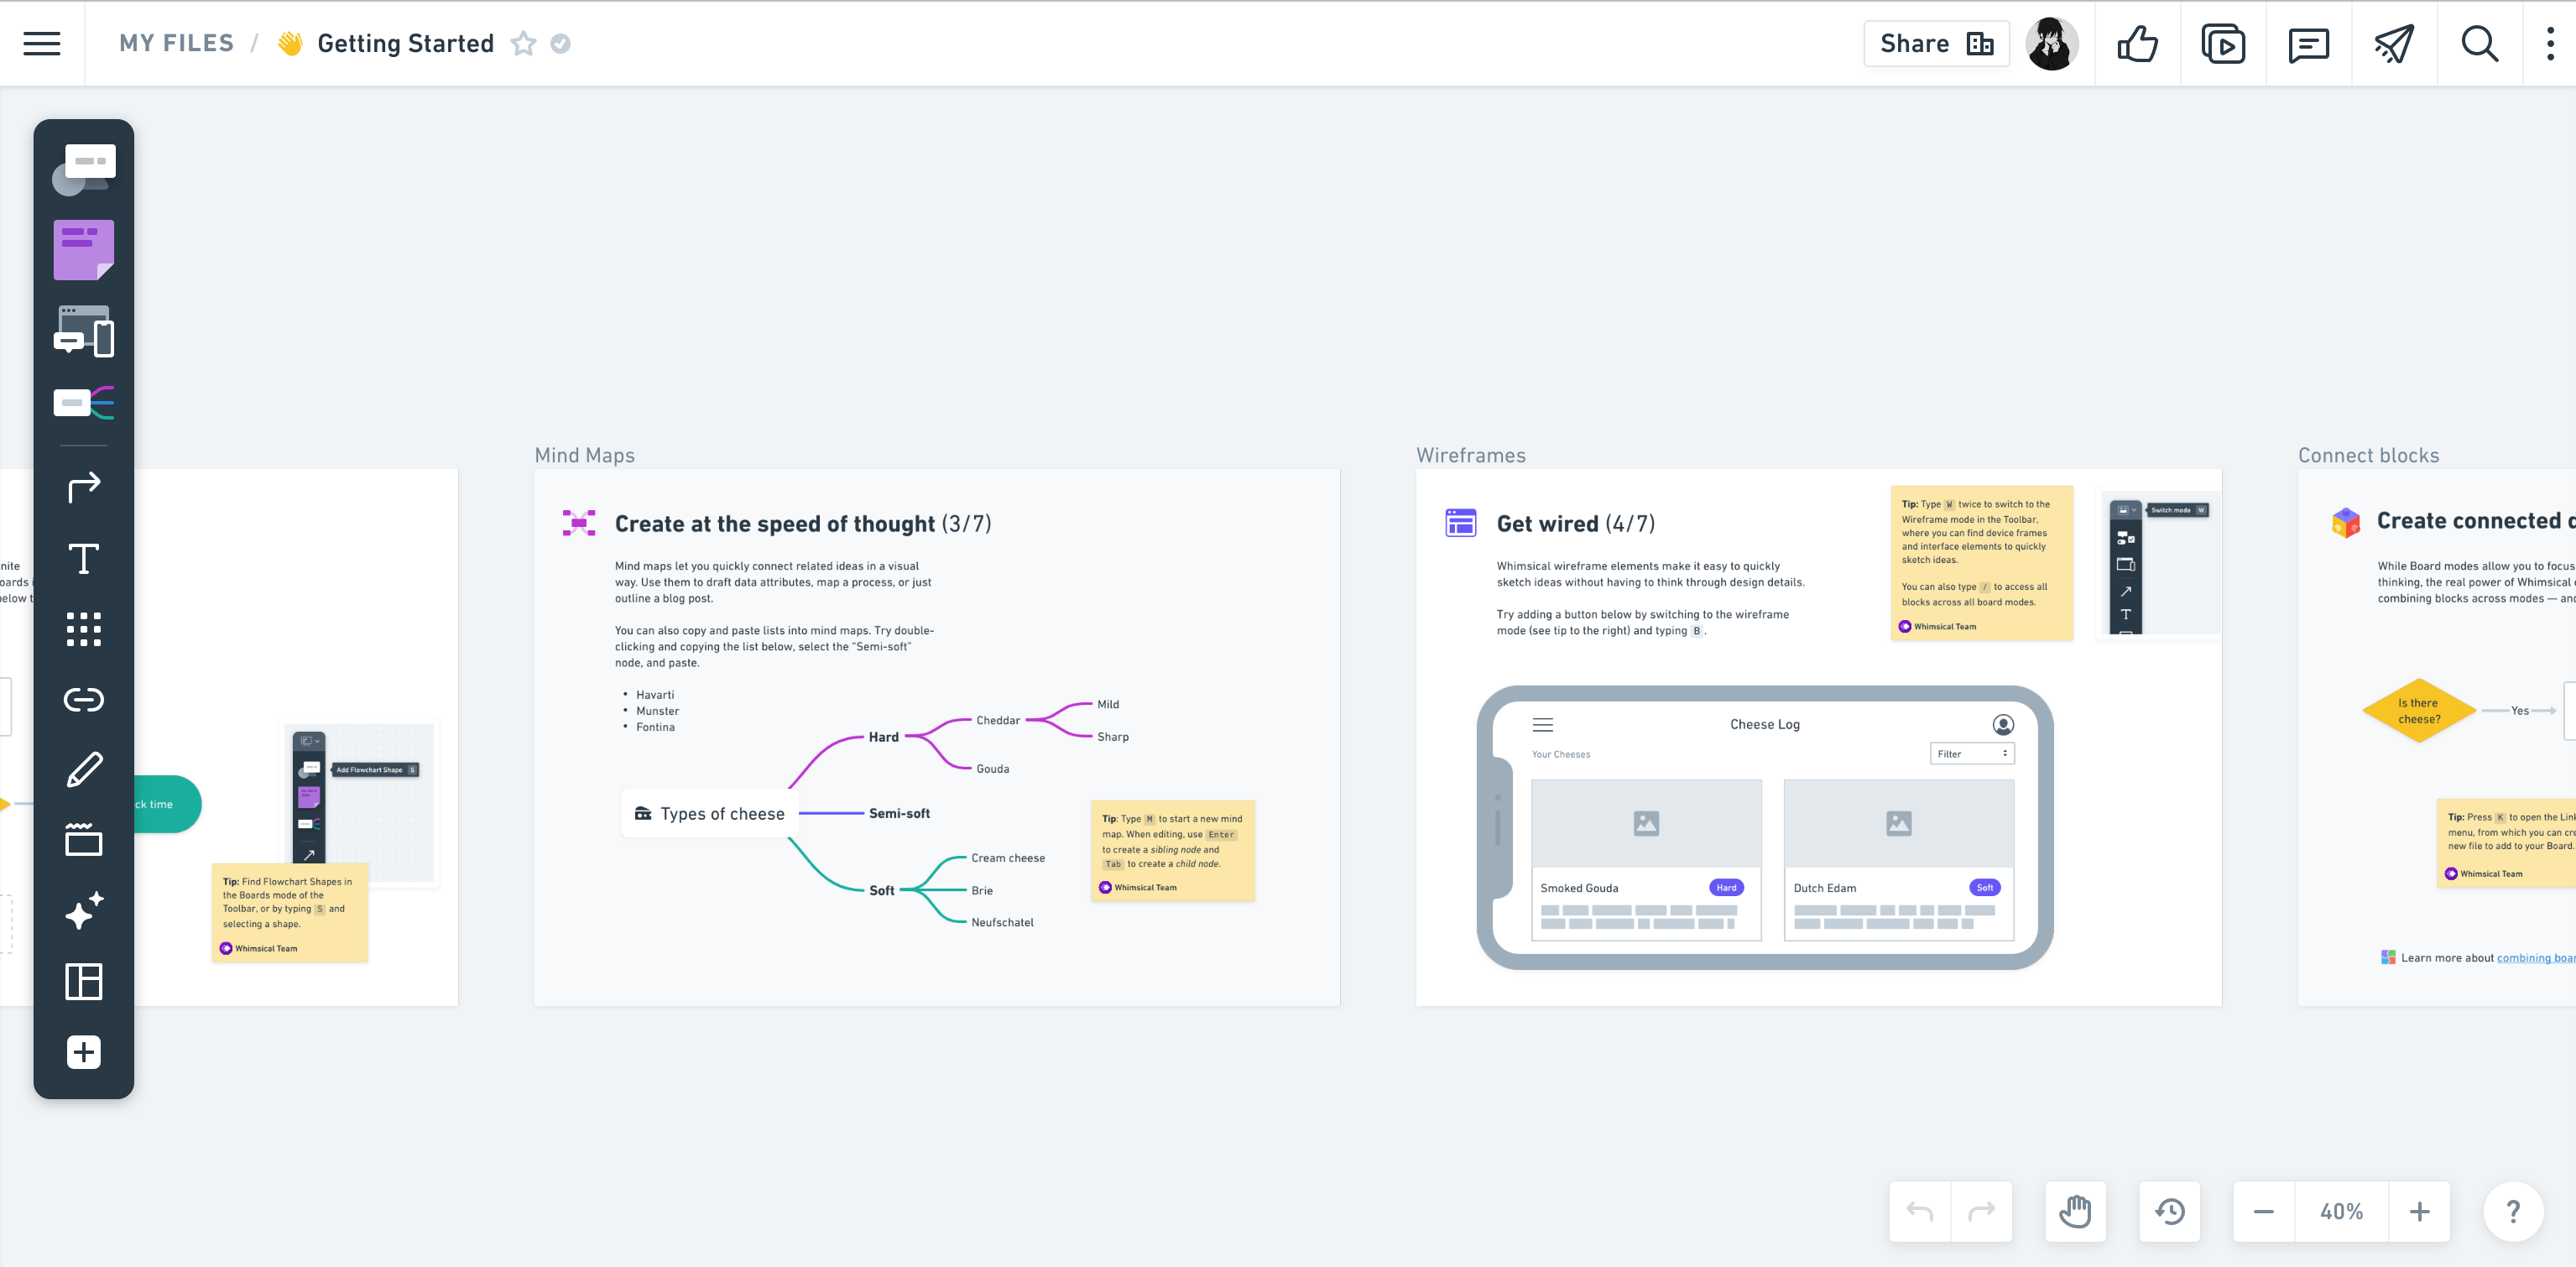
\includegraphics[width=.9\linewidth]{images/Captura de pantalla de 2023-08-19 17-35-40.png}
\caption{Pantalla inicial del Whimsical}
\end{figure}

\section{Conclusión}
\label{sec:orga4847d1}
Durante esta investigación, he aprendido nuevos conceptos como la investigación
de usuarios y la arquitectura de la información. También repasé temas que ya 
habíamos estudiado en cursos anteriores, como el diseño de interfaces de 
usuario. Creo que comprender cómo los usuarios interactúan con nuestra 
aplicación es fundamental para crear un producto de software exitoso. Además,
con las herramientas actuales, es posible lograr resultados profesionales en un
tiempo mínimo.


\pagebreak

\section{Referencias}
\label{sec:orgc01b4c6}
\printbibliography[heading=none]
\end{document}
